\chapter{مقدمه}

یادگیری تقویتی یکی از گرایش‌های یادگیری ماشینی است که از روانشناسی رفتارگرایی الهام می‌گیرد. این روش بر رفتارهایی تمرکز دارد که ماشین باید برای بیشینه کردن پاداشش انجام دهد. این مسئله، با توجه به گستردگی‌اش، در زمینه‌های گوناگونی بررسی می‌شود. مانند: 
\begin{alphinline}
	\item
	نظریه بازی‌ها،
	\item  
	نظریه کنترل، 
	\item 
	تحقیق در عملیات،
	 \item 
	نظریه اطلاعات، 
	\item 
	سامانه چندعامله، 
	\item 
	هوش ازدحامی، 
	\item 
	آمار، 
	\item 
	الگوریتم ژنتیک، 
	\item
	بهینه‌سازی بر مبنای شبیه‌سازی. 
	
\end{alphinline}

حوزه خودران سازی خودرو ها در سال های اخیر طرفداران زیادی پیدا کرده است. شرکت های بسیاری در دنیا مانند تسلا، رولزرویس، دیپ مایند، گوگل و اخیرا اپل، در حوزه حمایت‌های زیادی از این گونه فعالیت ها داشته اند. الگوریتم های یادگیری تقویتی از آن جهت در این بین محبوب است که یک ماشین سعی می‌کند مانند یک کودک، فعالیت کند و تجربه کسب کند و بیاموزد و حرکت کند. در واقع، قوانین به صورت امتیاز و یا پاداش به این سیستم وارد می‌شوند بدون آن که به ناظر نیاز شود.

این الگوریتم ها در دسته سوم شاخه های یادگیری ماشین، یعنی یادگیری تقویتی در کنار دو شاخه دیگر یعنی یادگیری با ناظر و یادگیری بدون ناظر مطرح می‌شوند. بر خلاف بخش های دیگهف این بخش ریاضیات قوی و کامل تری را شامل می‌شود. فرضیه ای در این حوزه به نام فرضیه امتیاز ها مطرح است که می‌گوید «همه اهداف را می‌توان با بیشینه کردن امید امتیاز های تجمعی توصیف کرد.»

در این پروژه سعی شد با استفاده از تعریف مناسب «مشاهده» و «امتیاز» ها و همچنین تعیین دیگر پارامتر های الگوریتم، به خودروی مورد مطالعه یاد بدهد که خودران شود. سرانجام این خودرو به صورت شبیه سازی شده شروع به حرکت کرد و مسیر را یاد گرفت.

به صورت کلی، این پروژه دو لایه کلی دارد؛ لایه الگوریتم و لایه شبیه ساز. 
لایه الگوریتم با استفاده از پایتون نوشته شده است اما لایه شبیه ساز با بکار گیری نرم افزار پری‌اسکن در محیط سیمولینک متلب این عمل صورت گرفته است. در حقیقت نوشتن یک محیط شبیه سازی (با قابلیت توسعه ساده در آینده)
از دستاورد های مهم و طاقت فرسای این پروژه می‌باشد.



همان‌طور که گفته شد، در این پروژه از ابزار های مختلفی استفاده شده است. برخی ابزارات دیگر نیز جهت ایجاد اتصال بین آن ابزار ها استفاده شده اند. در این بخش، این اجزا به تفصیل بررسی خواهد شد.

هر کدام از این اجزا کار مشخصی را بر عهده دارند.
شکل  
\ref{fig:block-diagram2}
این ارتباط را نشان می‌دهد.

\begin{figure}[h!]
	\centering
	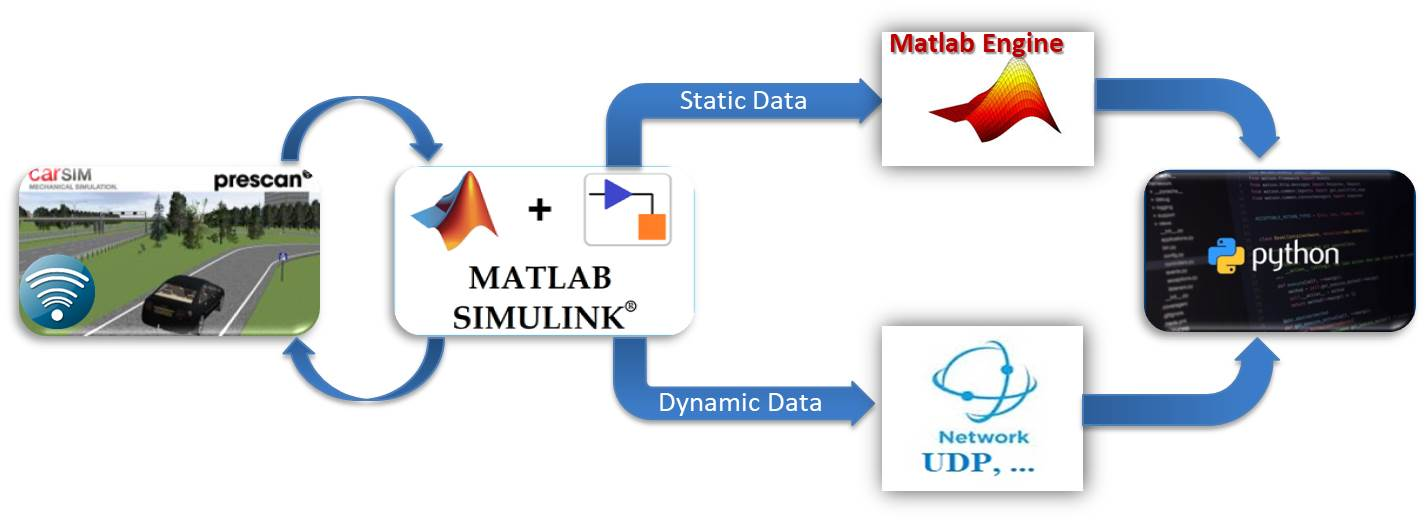
\includegraphics[width=1\linewidth]{Figures/block-diagram-white}
	\caption{بلوک دیالگرام لایه های کلی}
	\label{fig:block-diagram2}
\end{figure}

در شکل 
\ref{fig:block-diagram2}
از سمت چپ به راست اجزا یاد شده و نحوه ارتباط آن‌ها با‌یک‌دیگر را به‌خوبی نشان می‌دهد. این بلاک ها و ارتباط ها عبارتند از:

\begin{itemize}
	\item 
	اولین بلاک آن، نرم افزار \textbf{پری‌اسکن }می‌باشد. وظیفه اصلی این نرم افزار، شبیه سازی دینامیک یک اتومبیل و یا موتور و ... می‌باشد. همچنین ایجاد یک محیط گرافیکی زیبا و یک پنل کاربری گرافیکی برای ساخت ماشین ها از دیگر حسن های این نرم افزار است.
	
	فایل های مهم ایجاد شده توسط این بخش، \texttt{.pex} و \texttt{.pb} می‌باشد.
	
	\item
	بلاک بعدی ترکیبی از \textbf{متلب و سیمولینک }است. چرا که نرم افزار پری‌اسکن این امکان را دارد که برای کنترل و دسترسی بیشتر به قسمت های کنترلی مختلف، چیزی به نام \lr{API} ارائه می‌دهد. این \lr{API} یک فایل سیمولینک را در اختیار کابران قرار میدهد که در آن بلوک های مشخصی به یکدیگر متصل هستند و با مطالعه و تغییر آن بلوک ها می‌توان کنترل سیستم را به دست گرفت.
	
	فایل های مهم این بخش نیز در فرمت \texttt{.slx} و \texttt{.m} در دسترس هستند.
	
	همچنین \w{api} یاد شده، دستورات دیگری را جهت دریافت داده های استاتیک محیط ساخته شده در این نرم افزار را به کاربران خویش در محیط متلب می‌دهد.
	
	\item
	دو بلوک بعدی، مربوط به اتصال بین متلب و یا سیمولینک با پایتون هستند. 
	
	بلوک بالایی این اتصال را بین داده های استاتیک شامل طول جاده و عرض هر لاین، موقعیت اولیه اتومبیل و جاده، و بسیاری اطلاعات دیگر که بسیاری از آن اطلاعات استفاده نشده اند زیرا در این پروژه مفید نبوده اند. این بلوک، فایل سیمولینک را تغییر نمی‌دهد.
	
	بلوک پایینی نیز با استفاده از روش های شبکه کردن، می‌تواند داده های پویا را از محیط سیمولینک به پایتون منتقل کند. این داده های پویا عبارتند از موقعیت و سرعت و اطلاعات دیگری از اتومبیل در حال حرکت، اطلاعات سنسورها و ... باشد.
	
	\item 
	بلوک بعدی پایتون است که خود شامل لایه های دیگری است که در شکل 
	\ref{fig:python-layers}
	به تفضیل بیان شده است. نکته جالب در آن این است که در آن لایه ها اثری نیز از دو بلوک پیشین آمده است. همچنین بخش اصلی کار، یا به عبارتی مغز و هوش این کار در این قسمت توسعه یافته است.
\end{itemize}





در فصل \ref{ch:rl} توضیح بسیار مختصری در مورد خود مفاهیم یادگیری تقویتی می‌شود. فصل \ref{ch:resault} راه اندازی کد و نتایج حاصل این پروژه را نشان می‌دهد. پیش از راه اندازی باید باتوجه به فصل \ref{ch:req}، پیشنیاز های نصب آن تهیه و نصب گردند. همچنین آن فصل توضیح مختصری در مورد چیستی هریک از آن پیشنیاز ها ارایه کرده است. در فصل \ref{ch:alg}، نحوه تعریف پارامترهای الگوریتم یادگیری تقویتی به صورت کامل بسط داده شده اند. فصل \ref{ch:fani}، جزییات پیاده سازی محیط شبیه سازی را نشان می‌دهد و بر روی جزییات فنی آن تمرکز دارد.










